\cleardoublepage
\chapter{Resultater}
\label{chap:results} 

Dette kapittelet inneholder en presentasjon av produktet gruppen har utviklet. Her beskrives også gjennomførte evalueringer av arbeidet, selve produksjonen og hvordan dette ble gjennomført, hvordan resultatet ble og om det oppnådde krav og spesifikasjoner satt på forhånd.

\section{Presentasjon av produktet}
\label{section:presentasjon-produkt}
Produktet som arbeidet beskrevet i kapittel~\ref{chap:method} resulterte i er en prototype til tjenesten Aktiv Student i form av et prosjekt i Adobe XD. Prosjektet inneholder 42 sider med skisser laget av prosjektgruppen. Mange av disse skissene viser kun forskjellige valgmuligheter for samme funksjon og er derfor ikke nyttig å presentere i oppgaven. For å kunne vise skissene for alle de forskjellige sidene til tjenesten i bildeformat ble det valgt ut 20 skisser som alle ligger vedlagt i tillegg~\ref{vedlegg:skisser3}. Fem av disse skissene blir også presentert videre i delkapittel~\ref{section:presentasjon-produkt}.

For å kunne gi et bedre inntrykk av funksjonaliteten og navigasjonen i prototypen består produktet også av en video som viser en nøye gjennomgang av prototypen. Sammen med {\em anbefalinger for utvikling og videre arbeid} beskrevet i delkapittel~\ref{section:anbefaling-videre-utvikling} og andre retningslinjer gitt i dette dokumentet, leveres produktet til oppdragsgiver som et grunnlag for videre utvikling med instruksjoner og anbefalinger om hvordan formålet med tjenesten kan oppfylles.

\subsection{Minimalisme og konkretisering av informasjon}
En av de mest sentrale tilbakemeldingene fra initielle brukerintervjuer, beskrevet i delkapittel~\ref{section:init-brukerintervjuer}, var at deltakerne ønsket minimalistisk design og layout og kortfattede beskrivelser uten unødvendig informasjon. Disse tilbakemeldingene ble brukt som retningslinjer av prosjektgruppen under utviklingen av produktet. 

\paragraph{Beskrivende tekster}
I første forslag og skisser versjon 1.0, beskrevet i delkapittel~\ref{section:utforming-1}, forsøkte prosjektgruppen å unngå helt bruken av beskrivende tekster for å forklare funksjoner og elementer. Dette skapte forvirring hos deltakerne i brukertesten av skissene, som nevnt i delkapittel~\ref{section:Moderert brukertest-skisser-1}. I neste forslag og skisser versjon 2.0 bestemte prosjektgruppen seg for å inkludere beskrivende tekster der dette var påpekt som nødvendig, så lenge det ikke var mulig å tydeliggjøre funksjonene på andre måter. I brukertest av disse skissene, beskrevet i delkapittel~\ref{section:brukertest-skisser2.0}, kom det ingen tilbakemeldinger om at beskrivelsene var unødvendige eller brøt med det minimalistiske uttrykket. Prosjektgruppen bestemte seg derfor for å benytte beskrivende tekster der det var nødvendig i det ferdige produktet, men med så lite tekst som mulig. Beskrivelsene spilte også en rolle i å fremme en uformell og inkluderende tone, etter oppdragsgivers ønske nevnt i delkapittel~\ref{section:skisser1.0-oppdragsgiver}. Beskrivende tekst ble blant annet brukt på forsiden for å forklare kartleggingstesten, som vist i figur~\ref{fig:3-1-forside}.

\begin{figure}[H]
\centering
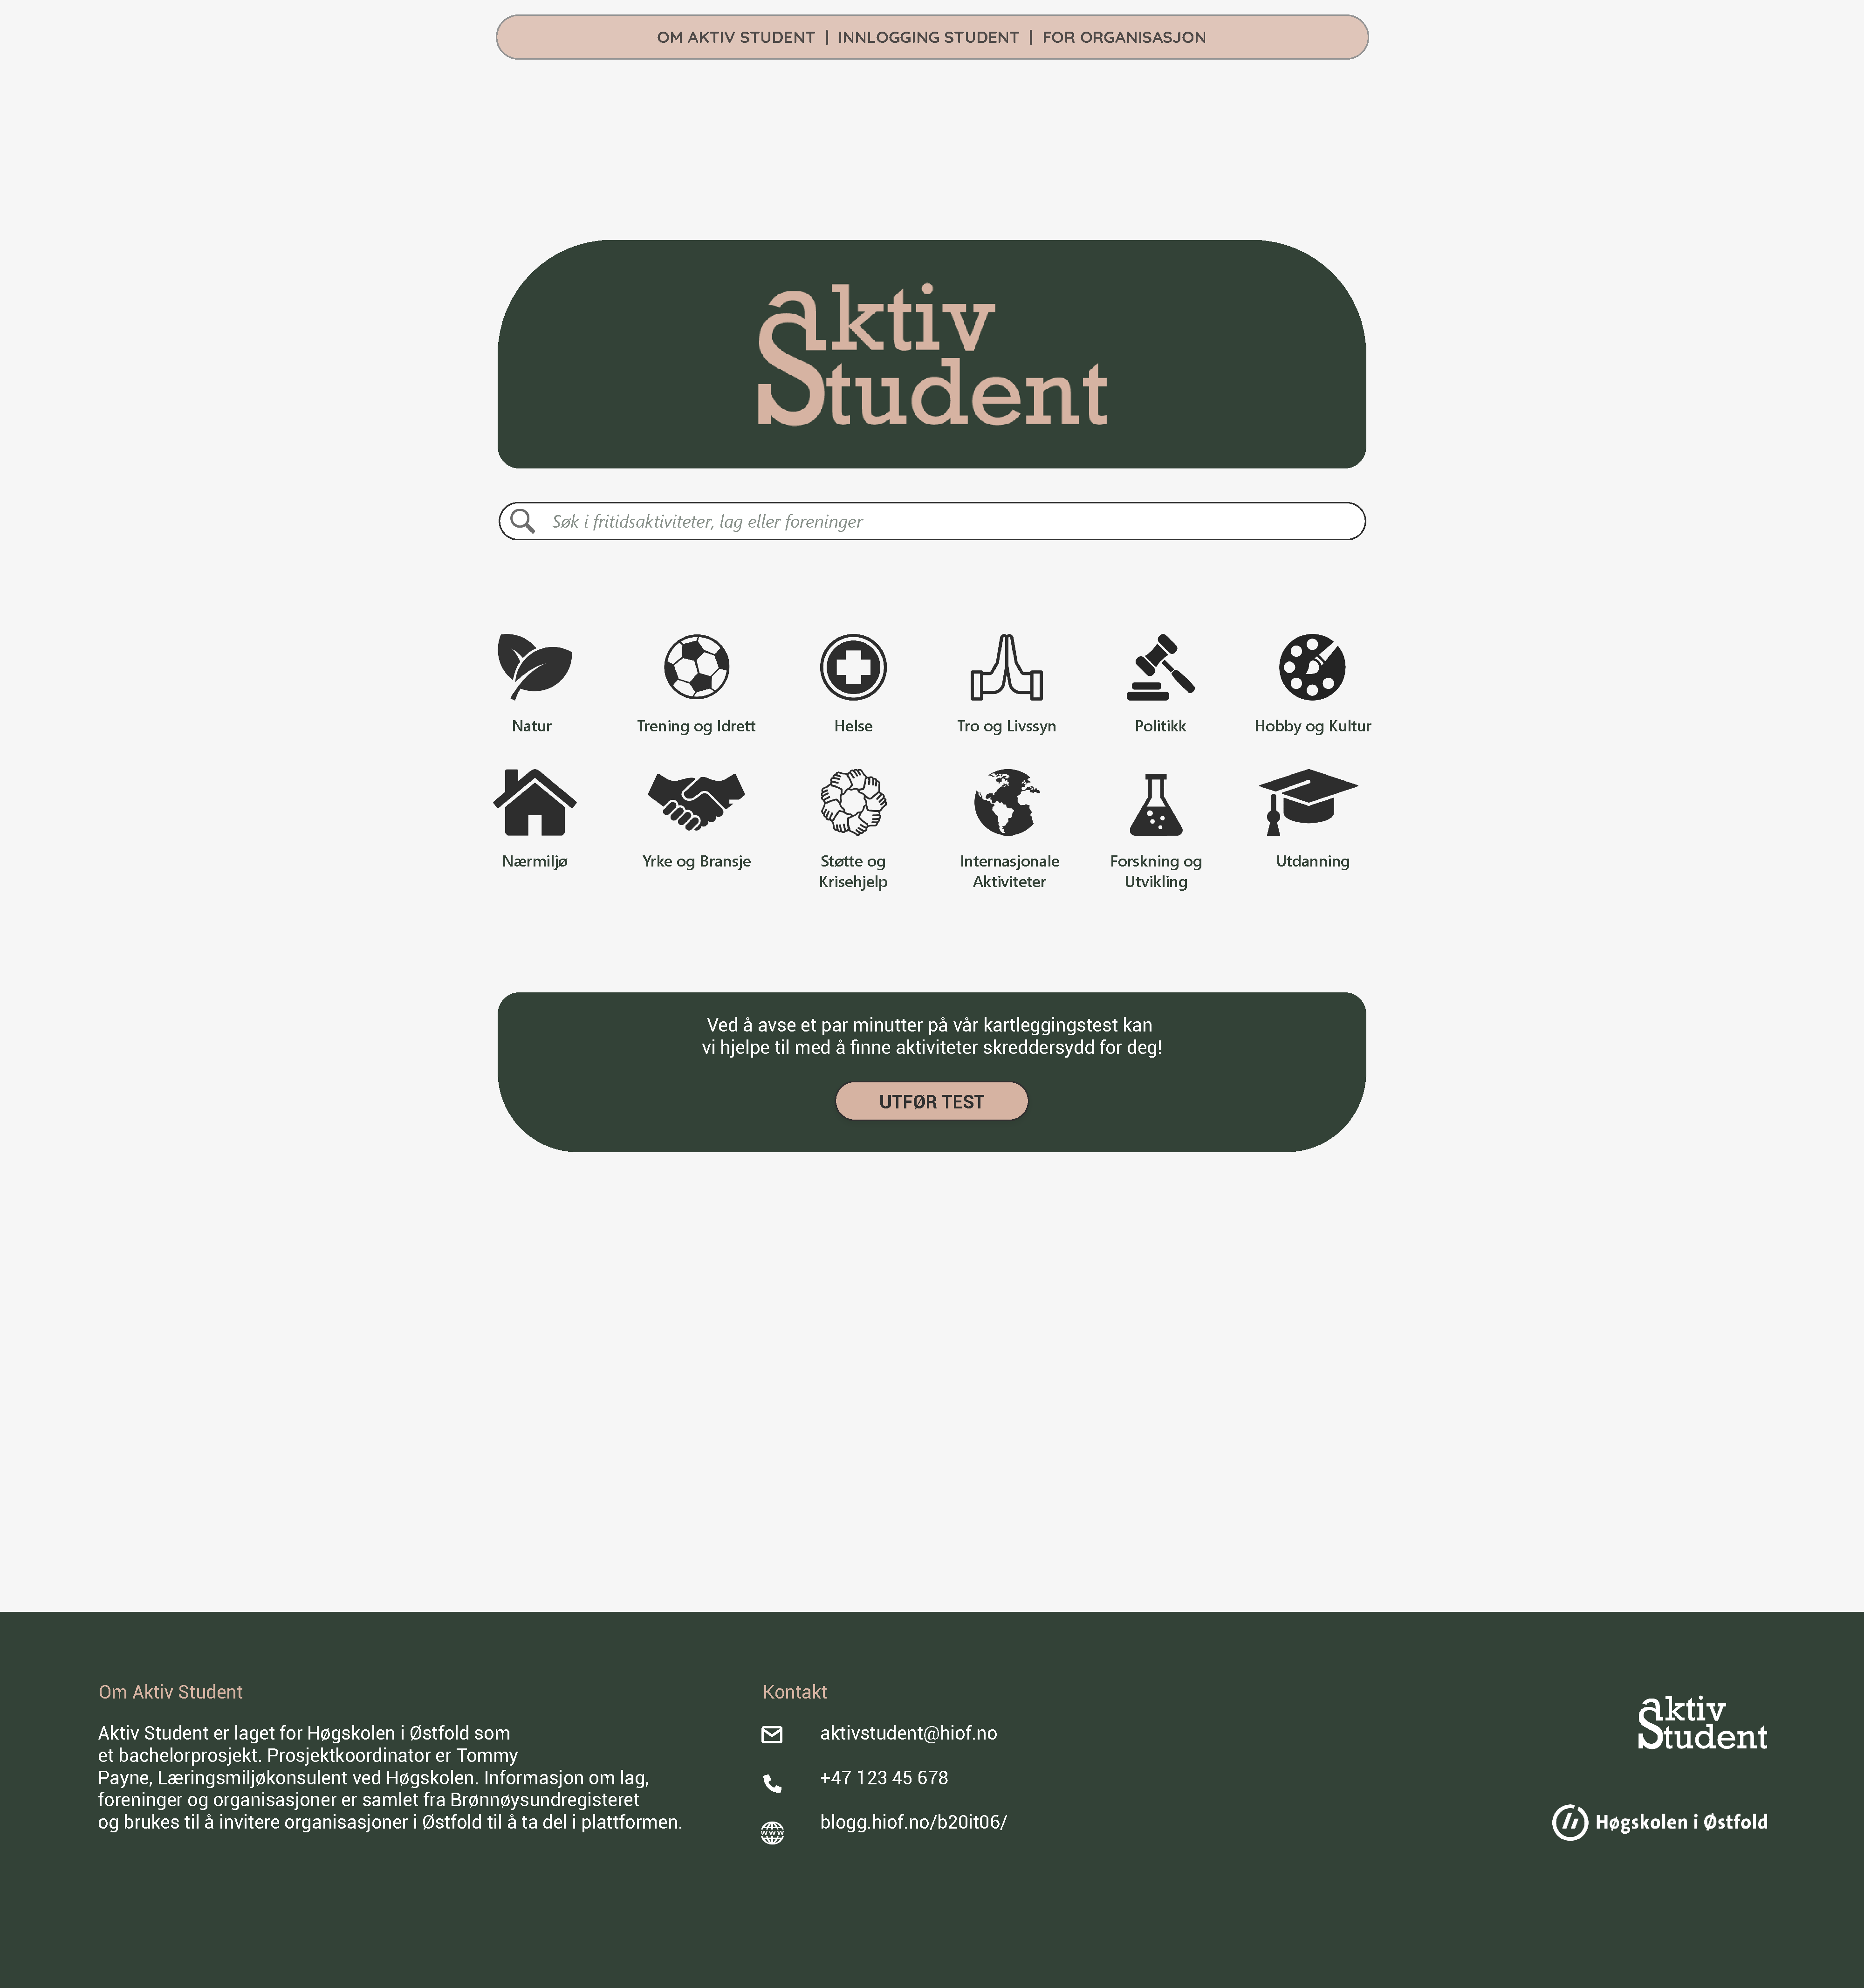
\includegraphics[width=.7\textwidth]{Illustrasjoner/Skisser-pdf/3.0/3-1-forside.pdf}
\caption{Adobe XD-skisse av plattformens forside}
\label{fig:3-1-forside}
\end{figure}

\paragraph{Layout og visuell design}
Valg innen plasseringen av elementer og design ble også gjort med tanke på minimalisme. Prosjektgruppen jobbet for å oppnå et layout som ikke virket rotete eller overfylt, med tydelige seksjoner for forskjellige elementer og en logisk plassering av elementer. Det ble eksperimentert med forskjellige mengder rom mellom elementene. I skisser med mye innhold var det viktig å ha nok mellomrom for å unngå at innholdet så tettpakket og rotete ut, men fortsatt ikke så mye mellomrom at brukeren kunne måtte scrolle langt ned for å finne innholdet den lette etter. Det ble også satt en standard for bredden på sidemargen, altså avstanden mellom innholdet og kanten av skissen. Denne bredden ble brukt på alle skissene som en kontinuitet og gjenkjennelighet i tjenesten, unntatt administratorpanel som var en selvstendig funksjon.

\paragraph{Logisk plassering av elementer}
Både i brukertest av skisser versjon 1.0, i del~\ref{section:test-forside-1.0}, og versjon 2.0, i del~\ref{section:test-forside-2.0}, ble plassering av elementer på forsiden tatt opp som et problem. Spesielt {\em ta testen}-knappen ble nevnt som et element som ikke hørte naturlig sammen med resten av innholdet i skissen og derfor burde flyttes lengre vekk fra de andre elementene. I utformingen av den endelige versjonen av forsiden, vist i figur~\ref{fig:3-1-forside}, ble {\em ta testen}-knappen og beskrivelsen flyttet til en egen seksjon på siden, med naturlig oppdeling fra de andre elementene.

\paragraph{Ryddig visning av resultater}
På skisser med resultatlister, som søkeresultater for organisasjoner eller aktivitetsvenner kom det tilbakemeldinger i brukertest av skisser 2.0 om at det så rotete og overfylt ut med tre knapper for hvert søketreff i listen, dette står nevnt i del~\ref{section:test-resultater-2.0}. For å skape en mer ryddig og minimalistisk oversikt ble knappene flyttet til en utbrettsmeny som kun vistes ved trykk på søkeresultatet i lista. I tillegg ble {\em kontaktinfo}-knappen fjernet ettersom kontaktinfo uansett sto på informasjonssiden. Hvert resultat i lista fikk også en egen boks med mellomrom imellom hvert resultat, i forsøk på å skape en ryddig og oversiktlig presentasjon av den viktigste informasjonen på siden. Den endelige skissen av siden for søkeresultater vises i figur~\ref{fig:3-3-resultater-filtrering}. Å bruke utbrettsmeny var en naturlig løsning for denne tjenesten siden utbrettsmenyer allerede ble brukt både på forsiden og i kartleggingstesten, disse tiltakene bidro derfor til å skape et konsistent design. Andre elementer i skissene som ble pekt på som dominerende eller ulogisk plassert i brukertestene ble også flyttet på eller endret størrelse på. For eksempel ble boksen med filtreringsmuligheter, også vist i figur~\ref{fig:3-3-resultater-filtrering}, gjort mye mindre og mer kompakt i den endelige versjonen av skissene i forhold til i skisser versjon 2.0. 


\begin{figure}[H]
\centering
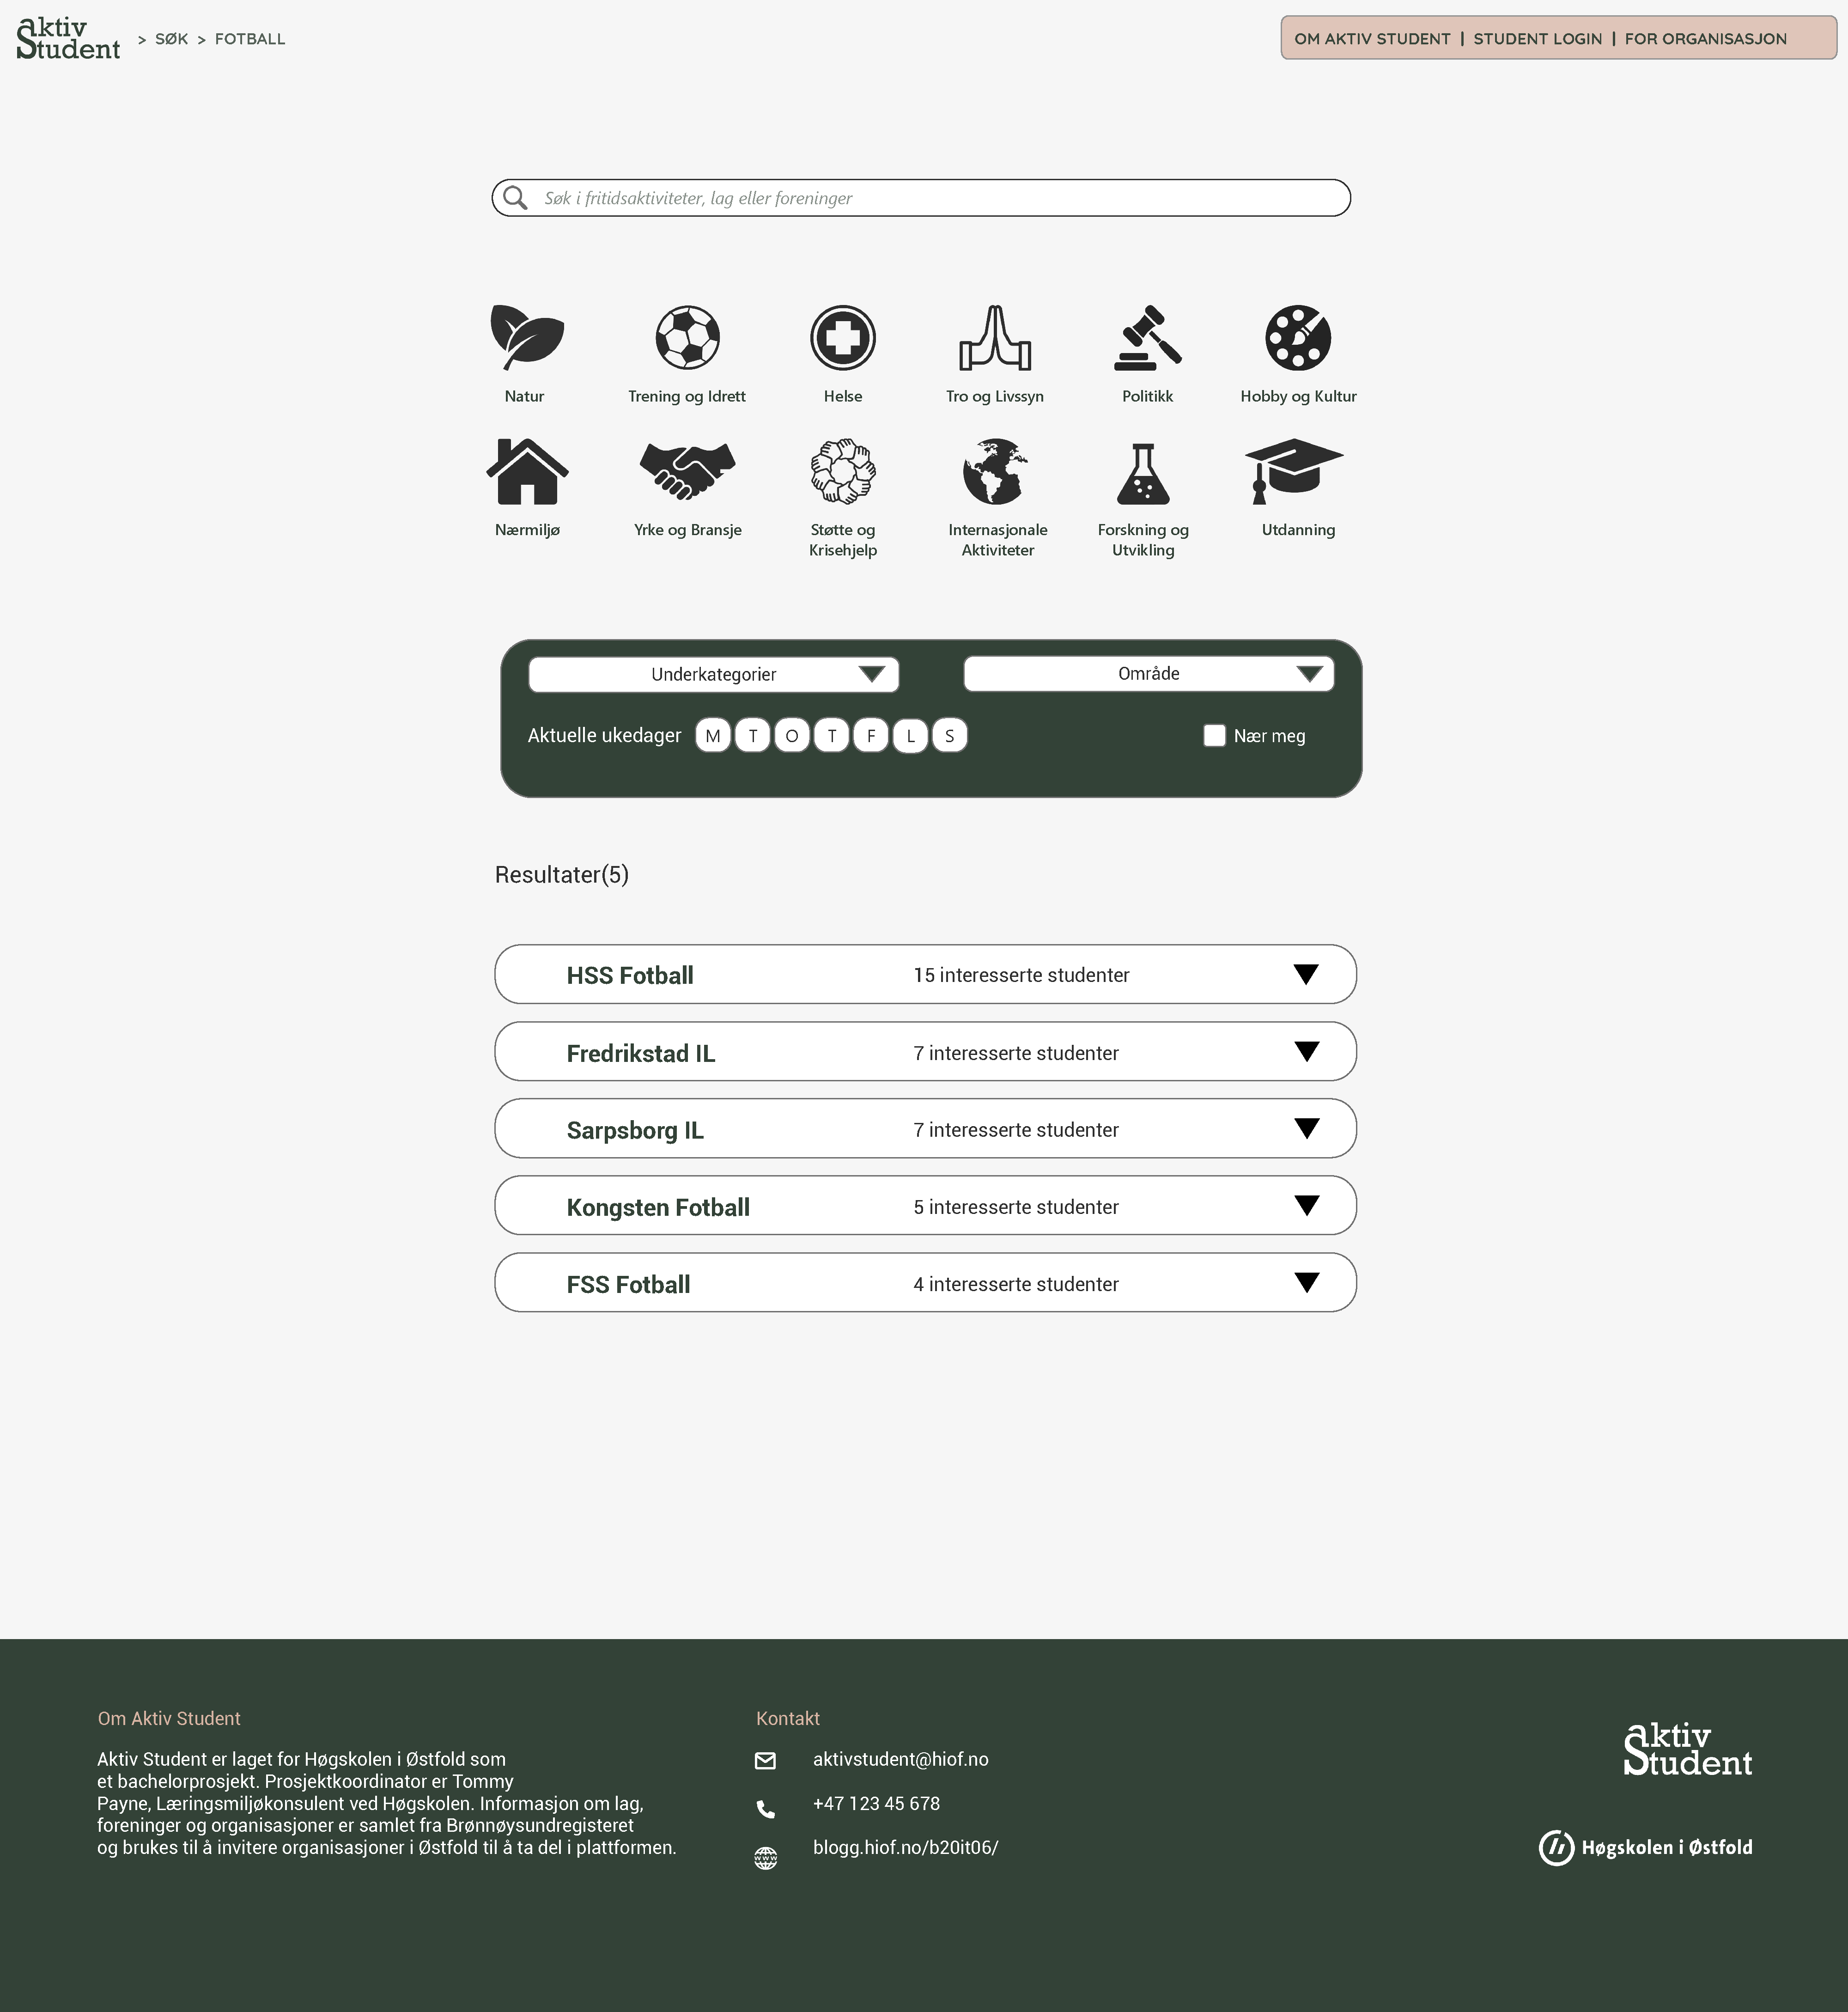
\includegraphics[width=.7\textwidth]{Illustrasjoner/Skisser-pdf/3.0/3-3-resultater-fotball.pdf}
\caption{Adobe XD-skisse av søkeresultatene etter bruker har trykket på underkategorien {\em Fotball}}
\label{fig:3-3-resultater-filtrering}
\end{figure}

\subsection{Navigasjon}
Skriv om logikken i navigasjon fra kategori til underkategori til resultater og bruk figur av forside med utbrettsmeny som eksempel. Dra inn begreper fra IA for navigasjon er sentralt der. Skriv om bruk av ikoner og bilder som visuelle virkemidler og hensikten med det (spennende, uformelt, lekent, blikkfang, gir et bedre inntrykk av innholdet på sidene man kommer til). Skriv om nav-bar i toppen, den tar ikke opp unødvendig plass, så mye luft på siden som mulig for lett og minimalistisk design.

\begin{figure}[H]
\centering
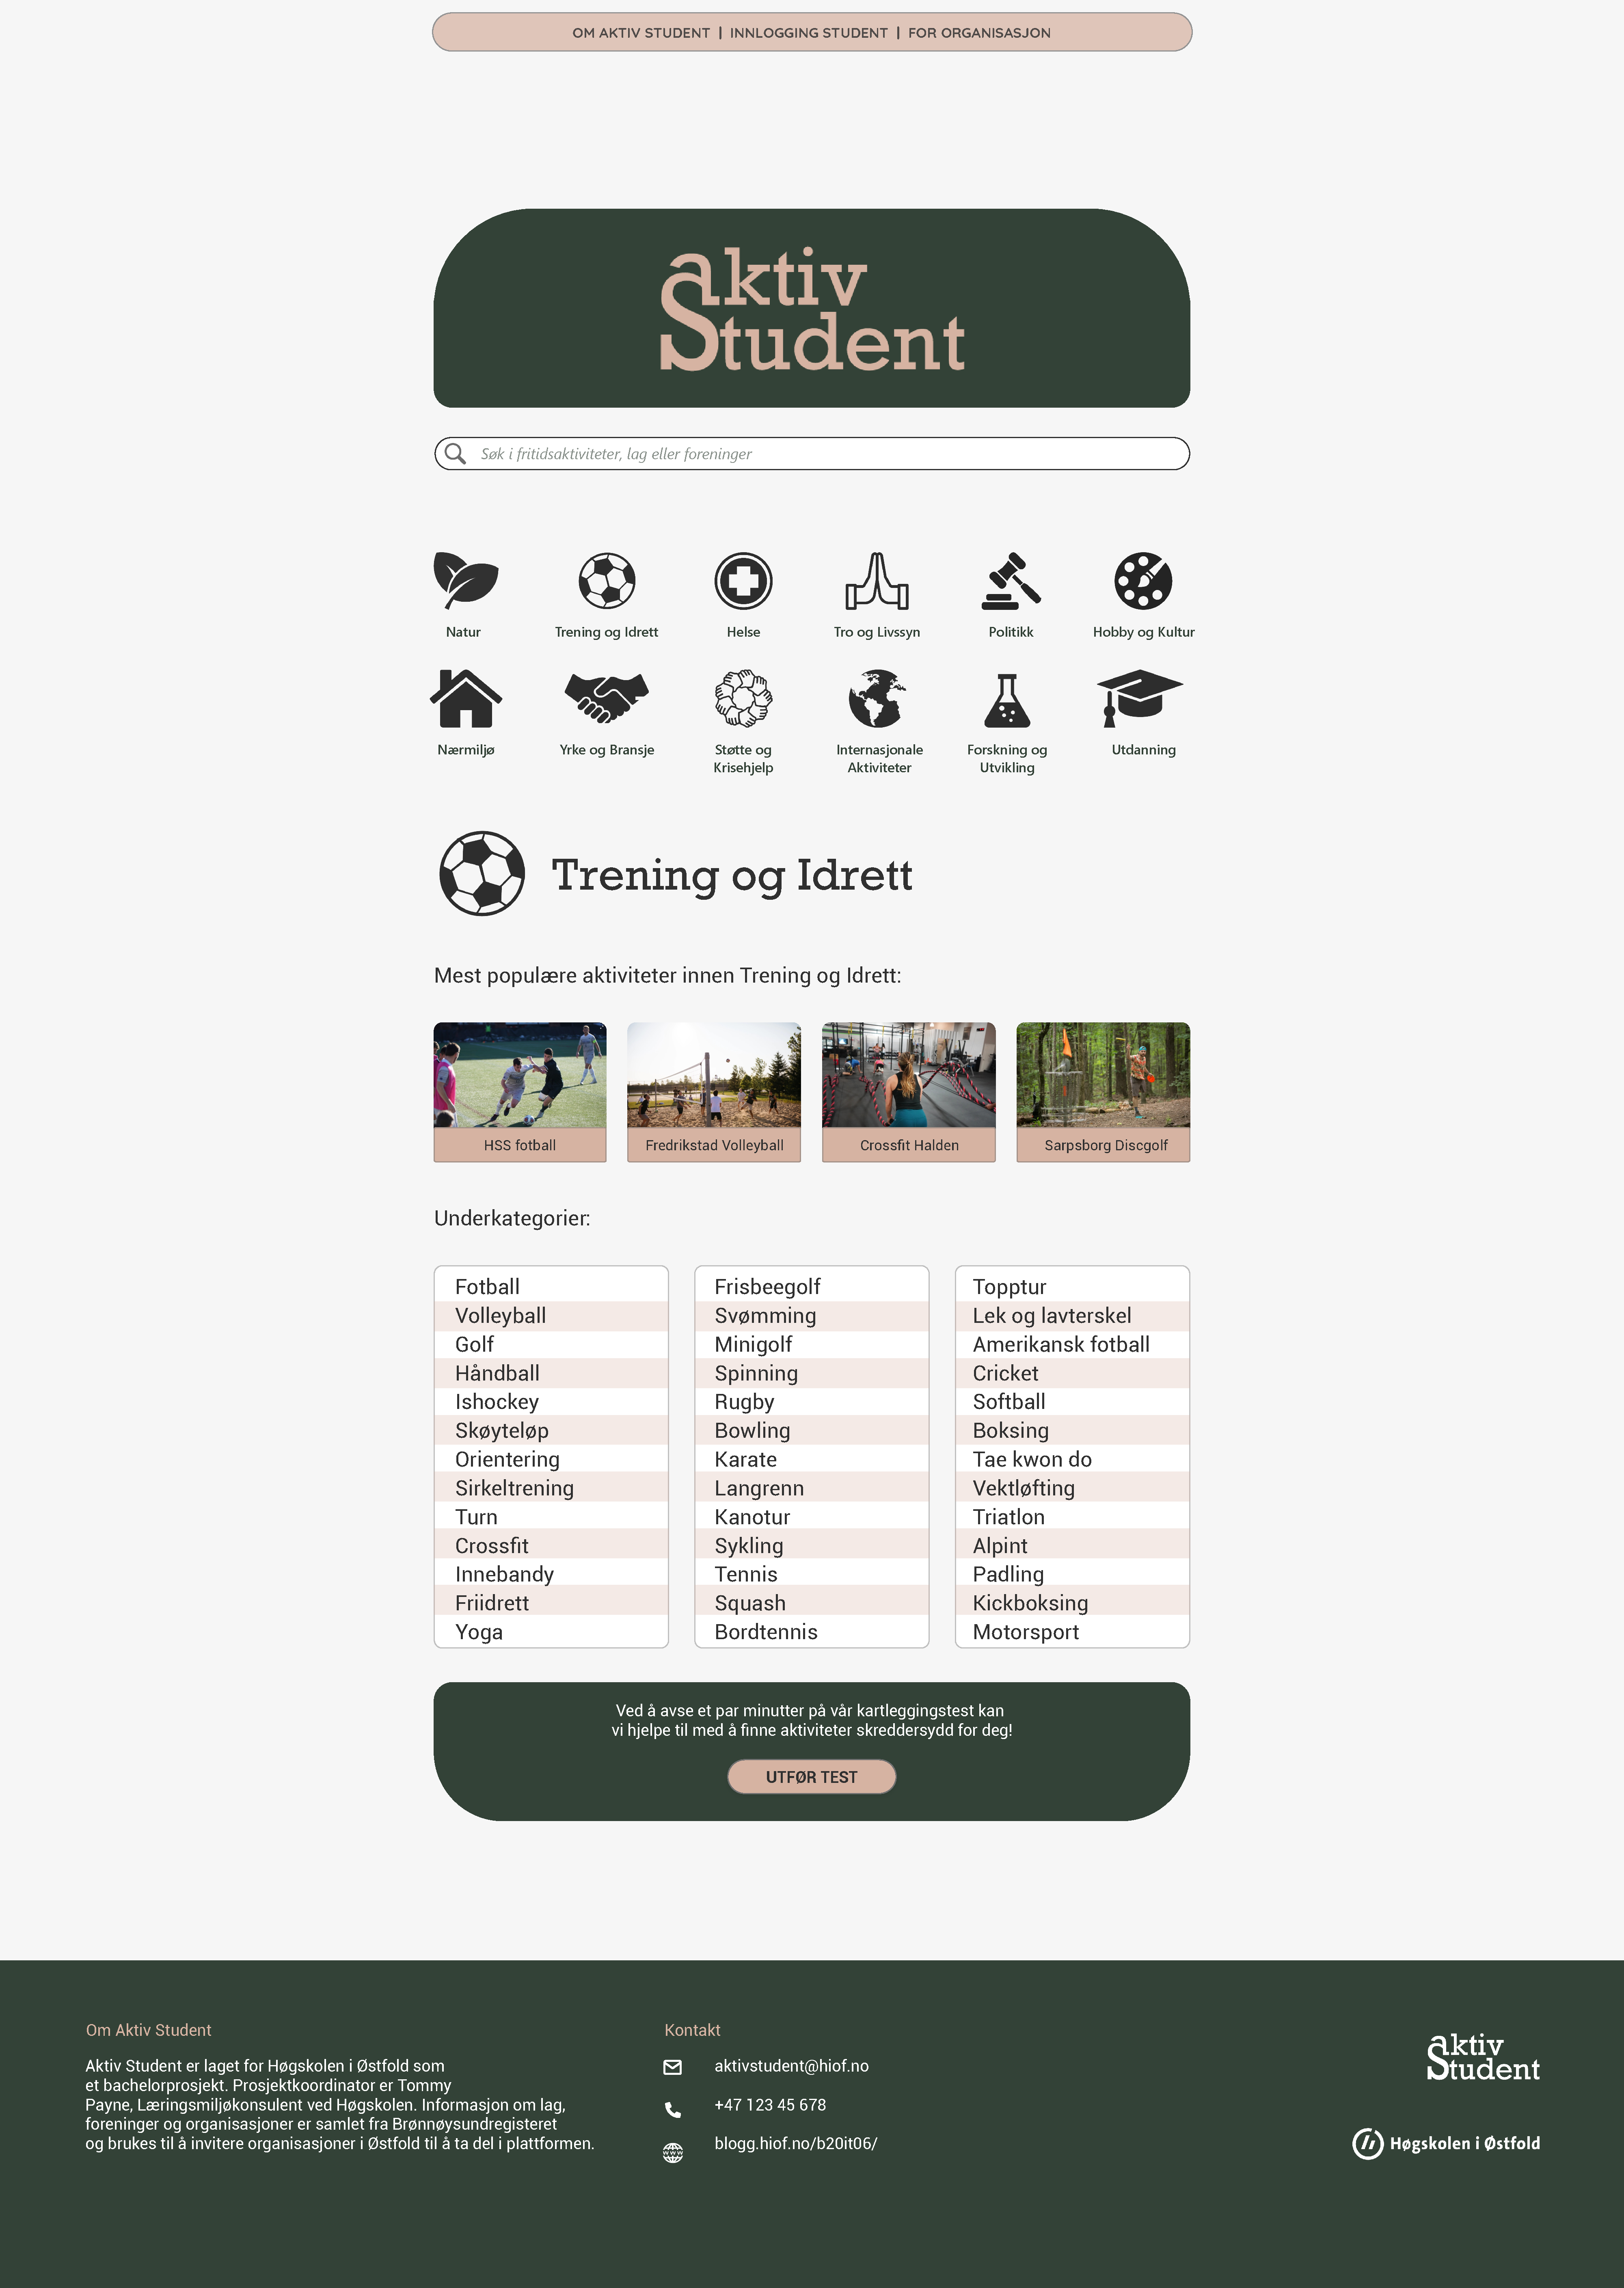
\includegraphics[width=.7\textwidth]{Illustrasjoner/Skisser-pdf/3.0/3-2-forside-trykket-kategori.pdf}
\caption{Adobe XD-skisse av plattformens forside etter bruker har trykket på kategori-ikonet for {\em Trening og Idrett}}
\label{fig:3-2-forside-utbrett}
\end{figure}

\subsection{Tilrettelegging for brukergenerert innhold}
Dette står det mye om i bøker om brukerorientert design, bruk kilder. Bruk organisasjonsside som eksempel på hvordan vi har tilrettelagt for at organisasjoner skal legge til utfyllende info om seg selv, knytte opp mot svar fra brukerintervju.


\begin{figure}[H]
\centering
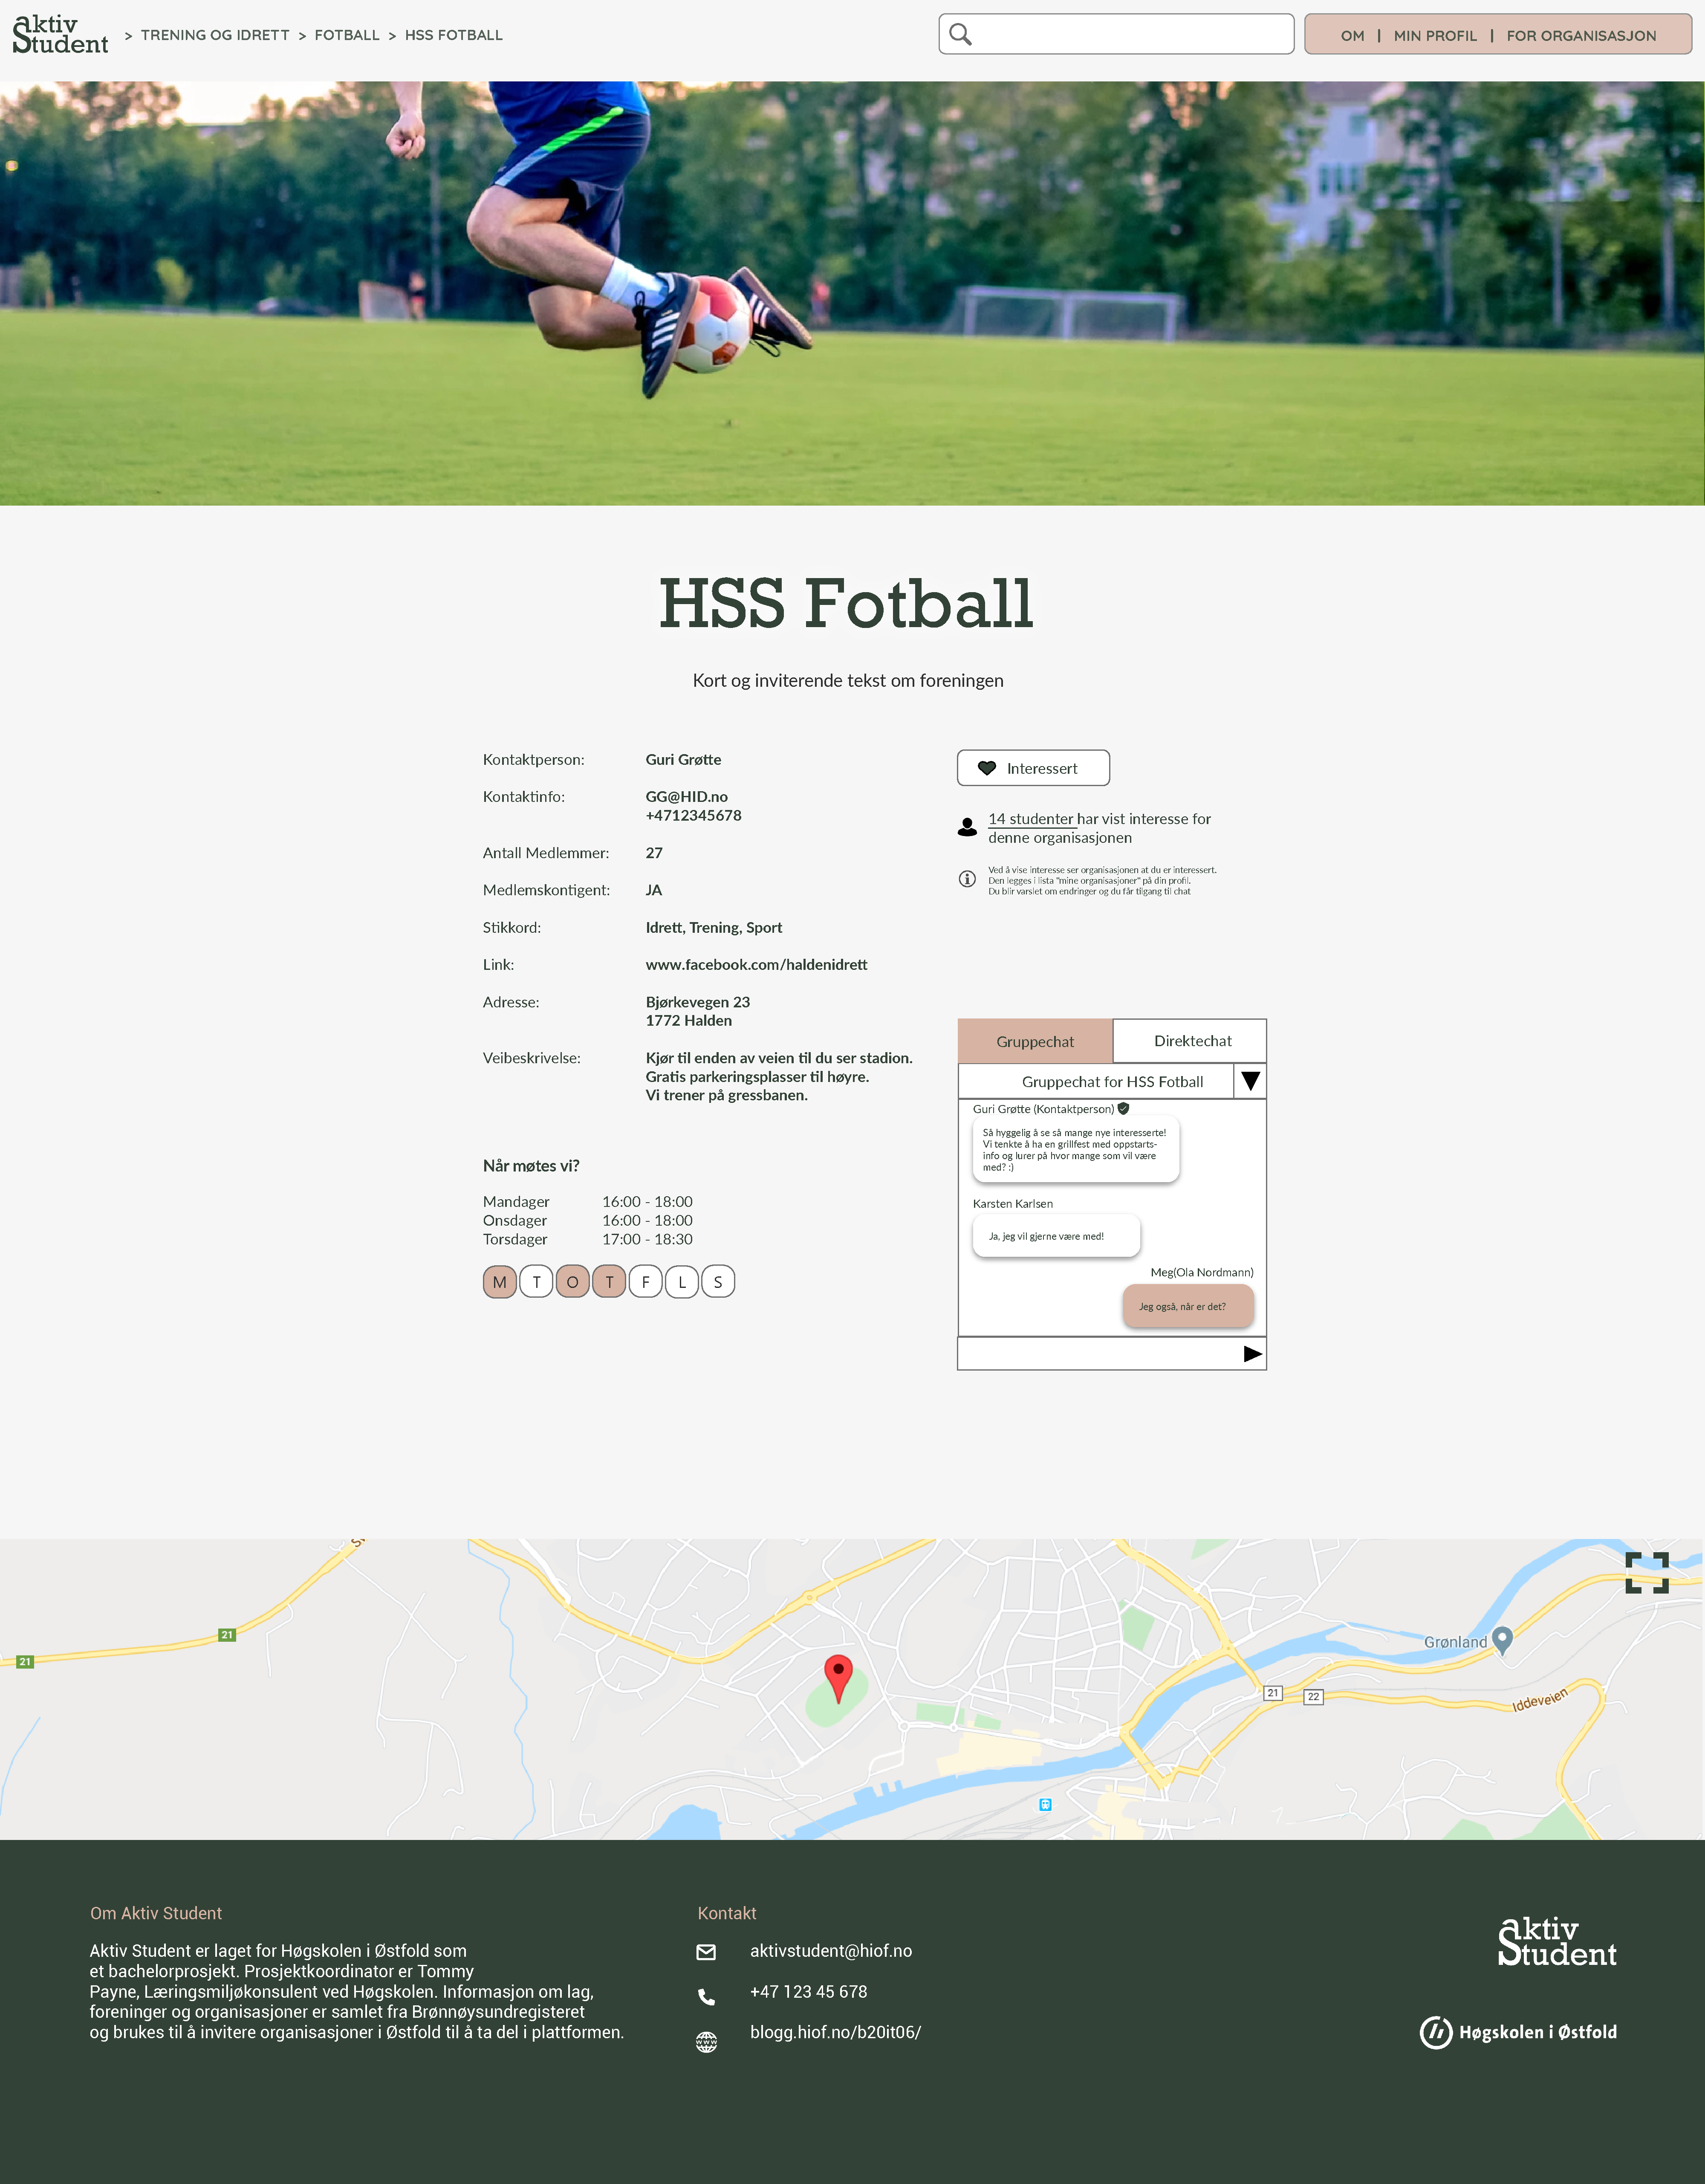
\includegraphics[width=.7\textwidth]{Illustrasjoner/Skisser-pdf/3.0/3-6-organisasjonsside-trykket-interessert.pdf}
\caption{Adobe XD-skisse av siden til eksempelorganisasjonen HSS Fotball etter bruker har trykket på {\em interessert}-knappen og får tilgang til chattefunksjonen}
\label{fig:3-6-org-trykket-interessert}
\end{figure}

\subsection{Spennende funksjonalitet}
Skriv om kartleggingstest og chattefunksjon og hele prosessen med dette. Skriv om hvordan det ikke bare er spennende men også kan hjelpe brukerne. Kartleggingstest som eksempel.

\begin{figure}[H]
\centering
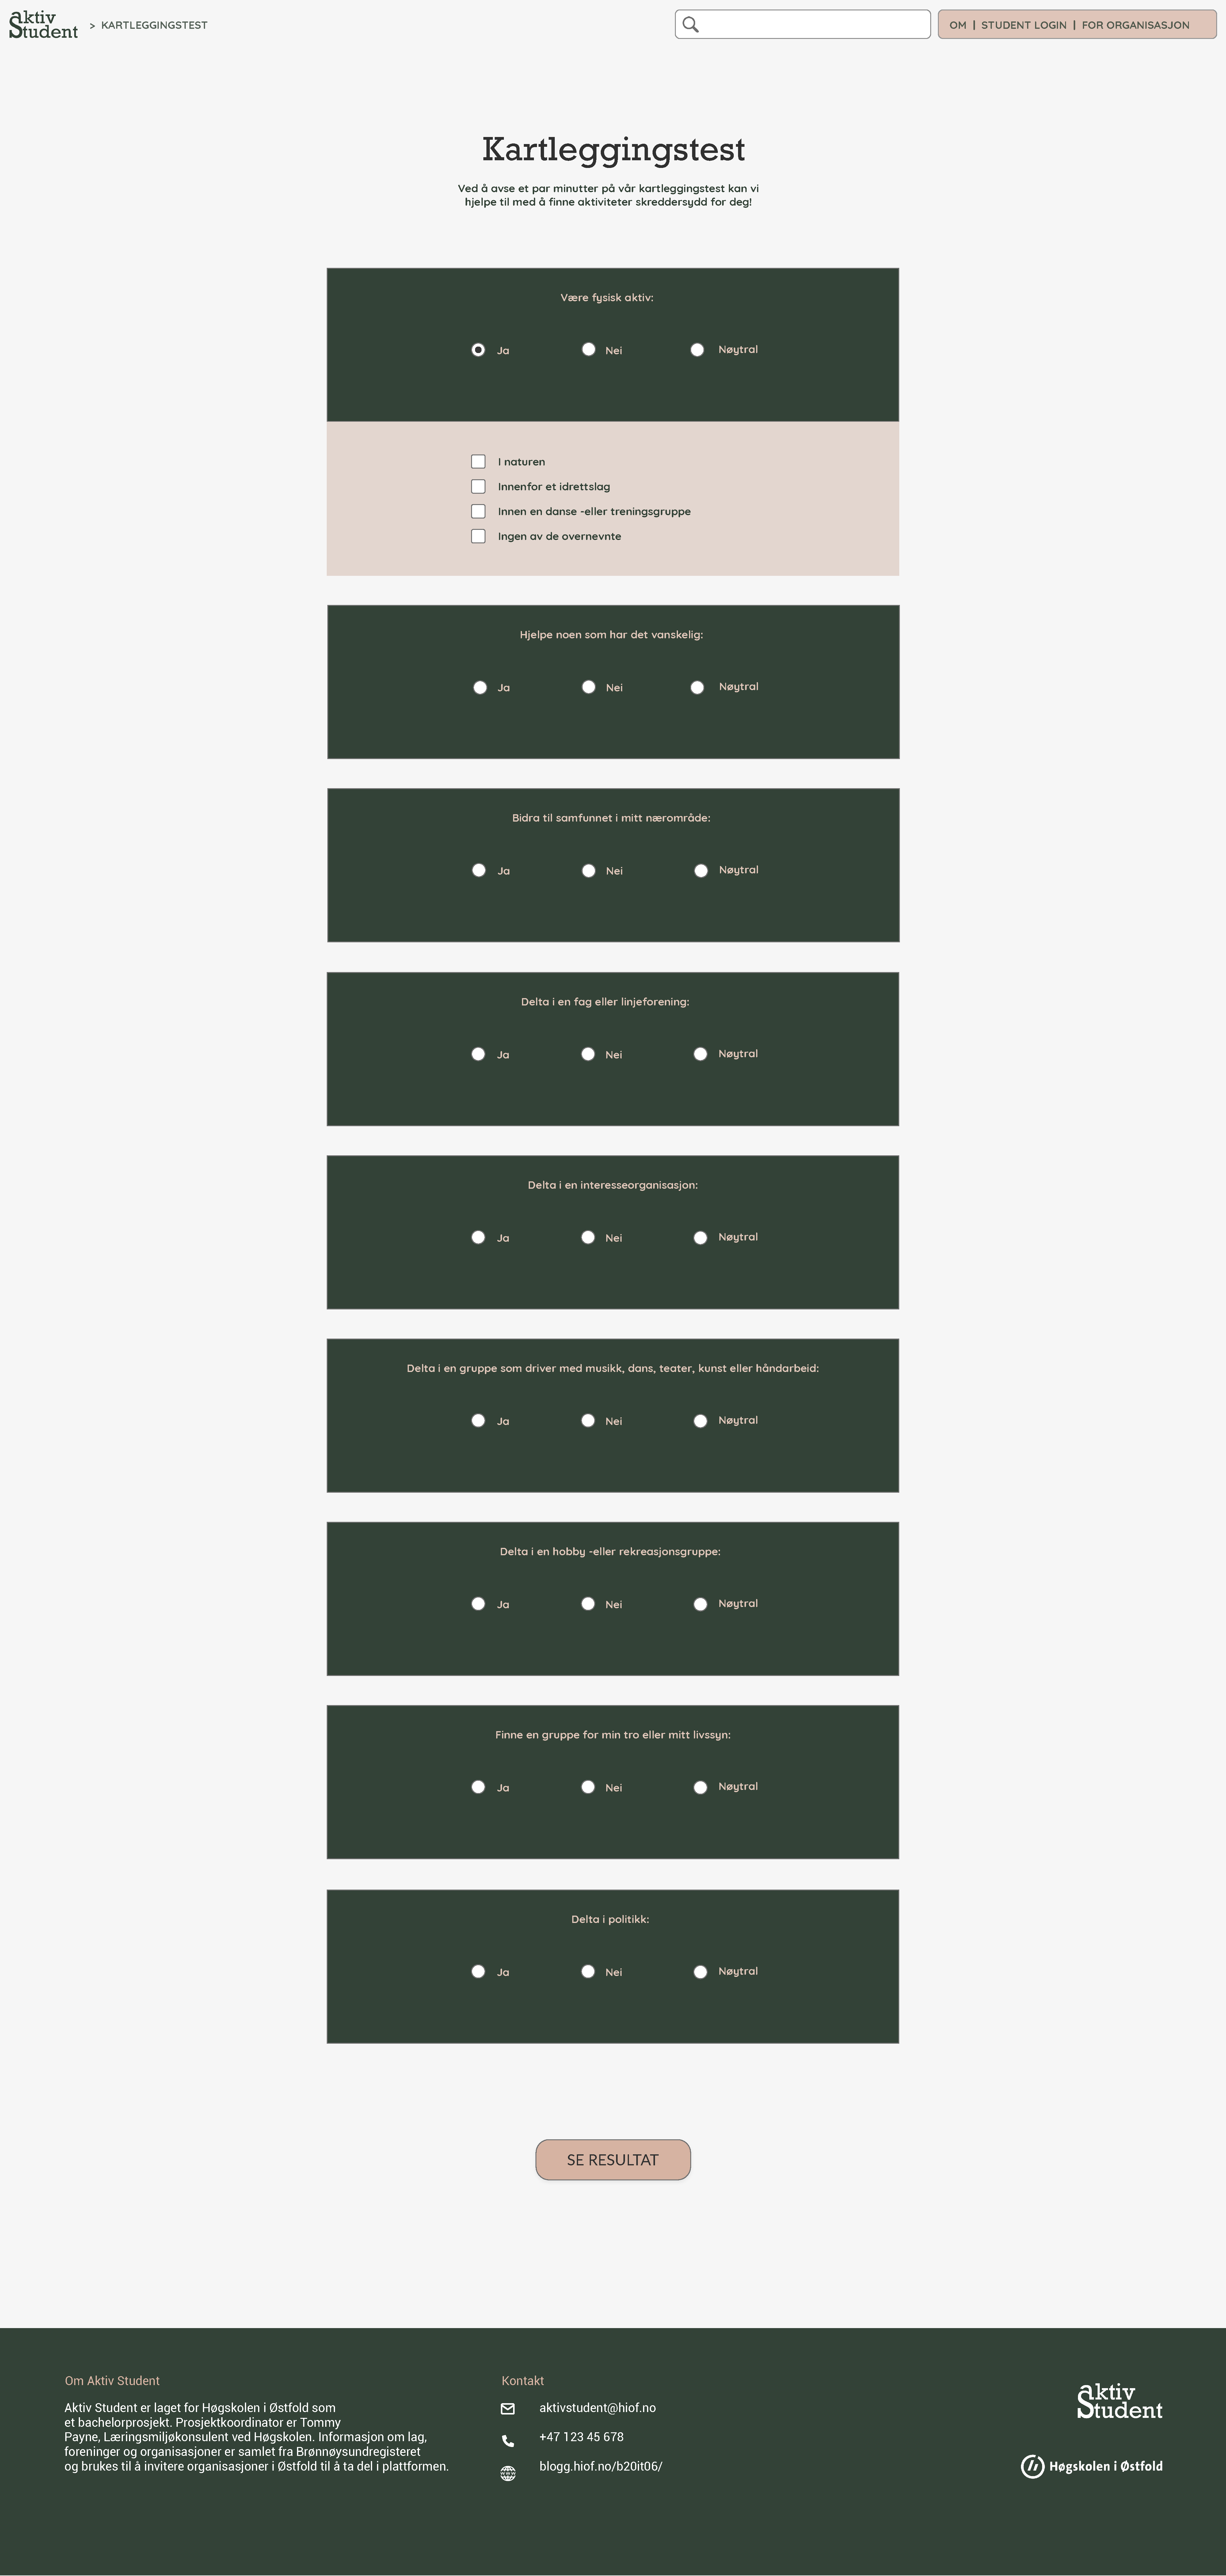
\includegraphics[width=.6\textwidth]{Illustrasjoner/Skisser-pdf/3.0/3-13-kartleggingstest-ved-svart-ja.pdf}
\caption{Adobe XD-skisse av kartleggingstesten med eksempelspørsmål etter bruker har svart {\em ja} på første spørsmål}
\label{fig:3-13-kartlegging-svart-ja}
\end{figure}

\section{Resultater fra undersøkelse av hypoteser}

De fire hypotesene som prosjektgruppen utarbeidet i begynnelsen av prosjektet ble undersøkt gjennom gruppens egne brukerundersøkelser, konsultasjon av fagpersoner og relevant forskning og faglitteratur. Dette ble gjort parallelt med arbeidet med produktet nettopp fordi hypotesene oppsummerte antakelser og spørsmål som prosjektgruppen ønsket å få svar på underveis i prosessen for å kunne utarbeide et godt produkt.

En sikker bekreftelse eller avkreftelse av hypotesene var enten ikke mulig eller ikke praktisk gjennomførbart for prosjektgruppen, men dette var heller ikke hensikten med hypotesene. Hypotesene ble brukt som en ledetråd for å finne de viktigste fokusområdene i videre undersøkelser og dermed i design av tjenesten. Det var derfor viktigst for prosjektgruppen å kunne bruke funn fra undersøkelsene i prosjektarbeidet og finne ut om funnene styrket eller svekket hypotesene, slik at fokusområdene eventuelt kunne justeres etter som.

\subsection{H1: En tjeneste som tilrettelegger for å delta sammen med andre likesinnede kan senke terskelen for å delta på en aktivitet}

\paragraph{Brukerintervjuer}
Hypotese 1 fikk støtte allerede under de initielle brukerintervjuene, beskrevet i delkapittel~\ref{section:init-brukerintervjuer}. 8/8 deltakere av brukerintervjuene svarte at å få med en venn eller bekjent ville gjort det enklere for dem å bli med på en organisert fritidsaktivitet. Dessuten svarte 7/8 deltakere at de tidligere hadde deltatt på en fritidsaktivitet fordi venner eller bekjente var med. De fleste av disse svarte også at det sosiale fellesskapet var en viktig grunn til at de valgte å delta. Noen svarte også at de ikke ville deltatt om de ikke hadde kjent til noen andre som deltok på aktiviteten.

\paragraph{Invitasjon til deltakelse gjennom mellomledd}
7/8 deltakere av de initielle brukerintervjuene svarte at gitt at de hadde en bekjent som var medlem i en organisasjon de var interesserte i, ville de tatt kontakt med den bekjente for å finne ut mer om organisasjonen. På den andre siden ville kun 2/8 deltakere tatt direkte kontakt med organisasjonen. Dette bygger opp under antakelsen om at personer i målgruppen heller ønsker å tilnærme seg organisasjonen gjennom et mellomledd enn å ta kontakt og delta alene. 

Dette ble gitt videre støtte av fagperson Anders Midtsundstad, som har utviklet metoden Fritid med Bistand \footnote{https://www.fritidmedbistand.no/}. Midtsundstad skrev i en samtale med prosjektgruppen via e-post at \say{I metoden Fritid med Bistand er det saksbehandler som har et ansvar i arbeidet med metoden til å legge til rette for deltakerne. Dette innebærer behov for å bruke den tid som kreves for å etablere tillit mellom metodens aktører. [...] I metoden Fritid med Bistand handler det om unge og eldre med ulike former for bistandsbehov. Studentene som er deres målgruppe har ofte en annen situasjon, men tillitsrelasjonen må en alltid forholde seg til. Det betyr i praksis at en tredjeperson bør invitere til fellesskapet} \cite{MIDTSUNDSTAD-EPOST:14}. 

Intervjuet med kvinnen som jobber i NAV indikerer mye av det samme. Kvinnen sa i intervjuet at \say{det kan virke som mange må ha noen som kan fysisk følge dem til arrangementer, ei hånd å holde i. Det hjelper ikke hvor mange tilbud man får når man er alene} \cite{NAV-INTERVJU:16}. Her var altså hjelp fra et mellomledd og deltakelse sammen med noen andre sentralt for at personene skulle tørre å dra på arrangementer. 

\paragraph{Konklusjon av undersøkelse av hypotese 1}
Etter undersøkelse av hypotese 1 kom prosjektgruppen fram til at ved å tilrettelegge i tjenesten for å delta sammen med andre eller å bli invitert til å delta av et mellomledd er det sannsynlig at dette kan føre til at studenter blir mer motivert til å delta. Gjennom at det sosiale og menneskelige aspektet ved tjenesten blir gjort tydelig kan studenten få større tillit til organisasjonen \cite{MIDTSUNDSTAD-EPOST:14}. Uten å utvikle tjenesten og teste denne i bruk er det dog umulig å si sikkert om tjenesten faktisk vil senke terskelen for å delta på aktiviteter, men prosjektgruppens funn styrker hypotese 1.

\subsection{H2: Studenter ved HIØ syns det er vanskelig å finne en oversikt over aktivitetstilbud}

\paragraph{Brukerintervjuer}
Svar fra de initielle brukerintervjuene støttet opp under hypotese 2. 6/8 deltakere svarte at å få bedre oversikt og tilgang til aktivitetstilbud ville gjøre det enklere for dem å delta på en aktivitet. Det som samtidig ble nevnt var vanskeligheten med å finne fram til kontaktinformasjon eller informasjon om hvordan man kunne delta på en aktivitet. 7/8 deltakere svarte at lett tilgjengelig kontaktinformasjon til organisasjoner spilte en viktig rolle i om de ville ta kontakt eller ikke. I tillegg svarte 8/8 deltakere at de ville tatt kontakt med en interessant organisasjon om det hadde eksistert gode tjenester som gjorde det enkelt å ta kontakt.

Deltakerne som ikke hadde deltatt på en organisert fritidsaktivitet i løpet av studietiden ble spurt om hva som holdt dem fra å delta. Én deltaker svarte \say{det er for dårlig tilbud. Jeg har sjekket tilbudet til HSS men ingenting der fenger.} En annen deltaker sa at han \say{vet ikke hva som er tilgjengelig og da gidder jeg ikke å begynne å lete.} Det ble også nevnt av flere deltakere at det var viktig for dem å ha lett tilgang til god og oppdatert informasjon om organisasjonene, ettersom flere av deltakerne heller ville lest om dem og møtt direkte opp på møte enn å tatt kontakt med organsasjonen først.

\paragraph{Mangler ved dagens aktivitetstilbud}
I alle rundene med brukerundersøkelser som ble gjennomført ble deltakerne spurt om sine tanker om konseptet Aktiv Student. Svarene som kom fram pekte på en mangel på et oversiktlig aktivitetstilbud for studenter ved HIØ i dag. I førsteinntykkstesten av skisser 1.0 sa en deltaker at han \say{liker konseptet, det er mangel på dette i dag og studenter ved høgskolen trenger det}. I brukertesten av skisser 2.0 ble en ny gruppe med deltakere spurt samme spørsmål. Det ble sagt av en deltaker at plattformen \say{svarer på et eksisterende behov ved høgskolen.} En annen deltaker sa at han ville brukt plattformen fordi \say{informasjon om organisasjoner på HIØ i dag er overfladisk og spredt overalt}.

Et viktig element i alle brukerundersøkelsene var at deltakerne skulle kunne snakke fritt og med så få føringer fra prosjektgruppen som mulig. Problemene med aktivitetstilbudet ble følgelig tatt opp på eget initiativ av studentene som deltok i undersøkelsene. Av mange deltakere ble denne problemstillingen også nevnt som første tema i samtalene om fritidsaktivitetstilbudet for studenter ved HIØ.

\paragraph{Konklusjon av undersøkelse av hypotese 2}
Etter å ha snakket med til sammen 13 forskjellige studenter ved HIØ, noen av dem i flere omganger, forelå det mange svar og bemerkninger som styrket antakelsen om at studenter syns at dagens aktivitetstilbud ved HIØ er mangelfullt og uoversiktlig. Samtidig kom det ingen svar som svekket antakelsen. Det faktum at deltakere tok opp problemene med tilbudet uten direkte oppfordring fra prosjektgruppen ga antakelsen ekstra tyngde. Ettersom prosjektgruppen kun hadde tilgang på en liten testgruppe kunne ikke hypotesen testes grundig nok til å kunne bekreftes, men undersøkelsene som ble gjennomført styrker hypotese 2.

\subsection{H3: Studenter ved HIØ syns terskelen for å selv ta kontakt med organisasjoner og aktivitetsgrupper er for høy}

\paragraph{Brukerintervjuer}
Svar fra de initielle brukerintervjuene ga blandende tilbakemeldinger. 6/8 deltakere svarte at det hadde gjort det enklere for dem å delta på en organisert fritidsaktivitet om det hadde vært lettere å ta kontakt eller om organisasjonen hadde initiert kontakt. I tillegg svarte kun 2/8 deltakere at de ville tatt kontakt om de hadde funnet en organisasjon de var interessert i. Dette så ut til å peke mot at deltakerne syntes terskelen var for høy til å ta kontakt, men på den andre siden var det flere som svarte at de heller ville ha deltatt direkte på en aktivitet med organisasjonen uten å trenge å ta kontakt først. Dette indikerte at det ikke var {\em for høy terskel} som var problemet for deltakerne, ettersom å delta på en aktivitet er et steg videre fra å ta kontakt.

\paragraph{Fagpersoner og forskning}
I intervjuet med kvinnen som jobbet med sosialhjelp i NAV ble det tatt opp flere punkter som var relevante for hypotese 3. Det ble tatt opp at flere av NAV-brukerne syntes det generelt var vanskelig å initiere kontakt, også med personer som jobbet i NAV. Hun opplevde ofte at hun måtte ta den første kontakten med brukerne fordi mange hadde {\em telefon-angst} og slet med å ta kontakt selv \cite{NAV-INTERVJU:16}.

Funn fra forskningsartikkelen {\em To Go or not to Go!: What Influences Newcomers of Hybrid Communities to Participate Offline} indikerte at en av årsakene til at brukere av tjenesten Meetup \footnote{https://www.meetup.com/} valgte å ikke delta på en aktivitet kunne være den sosiale distansen mellom aktivitetens vert og brukeren. Undersøkelsene i artikkelen kom blant annet fram til at om verten var en erfaren bruker av tjenesten var det mindre sjanse for at en nykommer ville delta på arrangementet. \say{Host tenure was represented as the log of number of days since joining the group; i.e. about 3 (2.7) extra days of group membership for event host in the group results to a decrease of 23\% in likelihood of a newcomer choosing the event as their first one to attend.}. En av anbefalingene nevnt i artikkelen for å motvirke brukerens følelse av sosial avstand var å tilby brukeren direkte kontakt med aktivitetens vert i tjenesten. \cite{NEWCOMERS:4:CT17}

\paragraph{Konklusjon av undersøkelse av hypotese 3}
Undersøkelsene av hypotese 3 pekte mot to forskjellige årsaker til at personer valgte å ikke ta kontakt med en organisasjon. En mulig årsak kunne være både at terskelen av ulike grunner var for høy, slik intervjuet med kvinnen fra NAV og funn fra forskningsartikkelen indikerte. En annen mulig årsak kunne være at de ikke så hensikten med å ta kontakt når de heller kunne møte opp direkte på møtet, som funn fra initielle brukerintervjuer indikerte. Prosjektgruppen valgte derfor å designe funksjonalitet med hensyn til begge disse mulige årsakene. Ettersom årsaken til at studenter ikke ville ta kontakt med organisasjoner var uklar og testgruppen samtidig var for liten for å trekke konklusjoner førte undersøkelsene til at hypotese 3 ble svekket. Fokuset ble skiftet fra {\em kontakt-aspektet} til å {\em legge til rette for at studenter skulle ha en mulighet til å enkelt og med lav terskel delta i organisasjoner.}


\subsection{H4: Spennende funksjoner og godt design skaper en tjeneste som studenter ved HIØ vil bruke}

\paragraph{Brukerintervjuer}
I de initielle brukerintervjuene ble deltakerne stilt forskjellige spørsmål om teknisk utforming og funksjonalitet i tjenesten Aktiv Student og generelt i nettbaserte tjenester. Ikke overraskende svarte 8/8 deltakere at gode og spennende funksjoner og design var en viktig faktor for dem i en tjeneste de skulle bruke. Deltakerne dro fram forskjellige konkrete funksjoner som var viktige for dem, de mest sentrale var {\em en velfungerende søkemotor} og {\em logisk fremstilling av kategorier}. Blant designaspekter som ble tatt opp var {\em minimalistisk design} og {\em kortfattet informasjon} de som ble nevnt som de viktigste av deltakerne. Alle disse aspektene kunne oppsummeres med at studentene ønsket at det skulle være enkelt å finne fram til resultatene man lette etter uten unødvendig bakgrunnsstøy.

\paragraph{Brukertest av skisser}
I løpet av brukertesting av skissene beskrevet i delkapittel~\ref{section:Moderert brukertest-skisser-1} og~\ref{section:brukertest-skisser2.0} delte deltakere sin mening om tjenestens funksjoner. I brukertest av skisser 1.0 sa en av deltakerne om den utbedrede versjonen av kartleggingstesten \say{den gjør plattformen mer spennende og er helt nødvendig for at ikke plattformen kun blir et register}. Et flertall av deltakerne i denne brukertesten svarte at de ville tatt kartleggingstesten som første handling i tjenesten om den hadde vært ferdig utviklet. I brukertestene av skisser 1.0 og skisser 2.0 handlet de fleste av tilbakemeldingene om design og utforming. Plassering av elementer, tydeliggjøring av beskrivelser og mengden innhold på siden var områder som fikk mange tilbakemeldinger. Dette indikerte at godt design og utforming var viktig for studentene som deltok.

\paragraph{Designprinsipper og retningslinjer fra faglitteratur}
I boken {\em Designing for User Engagement on the Web: 10 Basic Principles} skrev forfatteren om hvilke designprinsipper som kunne benyttes for å skape en engasjerende brukeropplevelse i en nettbasert tjeneste. I boken ble interaksjon trukket fram som et viktig prinsipp: \say{People want to be active participants in communication, not just passive receivers of information.} (s. 71). I tillegg ble det gitt anbefalinger for økt brukervennlighet som gjenkjennelig design, lettleselig innhold og bruk av visuelle virkemidler som bilder og fonter for at brukeren skulle enkelt kunne finne ut hvilket innhold som var viktig for den \cite{ENGAGEMENT-WEB:17}. 

Boken {\em Successful User Experience: Strategies and Roadmaps} nevner kreativitet og innovasjon som viktige verktøy når det kom til å løse en brukers problem. Forfatteren skriver at for å finne innovative løsninger i design av brukeropplevelser må man tenke utenfor boksen \cite{SUCCESSFUL-UX:18}. Forfatteren av boken {\em Interactive Design : An Introduction to the Theory and Application of User-centered Design} skrev om hvordan underholdende og morsom funksjonalitet kunne engasjere brukeren og at prinsipper fra spill og lek kunne inkorporeres i oppgaver som vanligvis ville vært kjedelig å utføre: \say{Users are engaged through entertainment. the more pleasure a user gets from interacting with what you’ve designed, the more engaged they will be and the more likely they will be to return.[...] Good design itself can be pleasurable.} (s. 123) \cite{INTERACTIVE-DESIGN:19}.

\paragraph{Konklusjon av undersøkelse av hypotese 4}
Selv om antakelsen om at brukere av en tjeneste ønsket spennende funksjonalitet og god design kunne virke selvsagt valgte likevel prosjektgruppen å undersøke den. Hensikten med dette var å finne ut mer spesifikt hvilke faktorer som kunne gjøre en funksjon spennende og skape et godt design. Om implementasjon av prinsipper og retningslinjer funnet under undersøkelsene faktisk ville øke studenters motivasjon til å benytte tjenesten var ikke mulig å finne ut uten å gjennomføre og teste dette. Like fullt pekte svarene i de initielle brukerintervjuene mot at deltakerne la stor vekt på et godt design. I tillegg reagerte deltakerne positivt på foreslåtte spennende funksjoner i brukertestene av skisser. Faglig litteratur om brukerorienterte designprinsipper støttet også opp under antakelsen. Dette førte til at hypotese 4 ble styrket.


\section{Testing og evaluering}
%Hva ville vi få ut av testingen? Vite om produktet oppfylte krav og forventninger. Tips til videre utvikling og markedsføring%

\subsection{Teknisk funksjonalitet}
%Testing av skissenes funksjonalitet på 3 deltakere (Ingrid)%

\subsection{Studenters vurdering}
% Skriv litt om hensikten med undersøkelsen og gjennomføringen %
% beskrivelse av testdeltakere: kjønn, alder, bakgrunn, studiesituasjon, andre ting? %
% sitat pakkes inn i \say{sitat her} %
Deltaker 1 er en mann som bor ved og studerer ved Campus Horten. Han studerer en master i Maritim ledelse og gikk 1.året når testen ble utført.

Deltaker 2 er en mann som bor på kråkerøy og studerer Økonomi og administrasjon og gikk 2.året når testen ble utført. %var det slik du tenkte at det skulle bli skrevet?%
%Spørsmål stilt til studenter%
\paragraph{1. Finner du konseptet bak dette produktet interessant og brukbart og er dette noe du ville selv brukt?}
%oppsummering av svar fra alle%
Deltakerene syntes at konseptet hørtes interessant ut og tror det kan bli nyttig for mange studenter. De fleste deltakerene ville prøvd plattformen om det hadde vært tilgjengelig på deres studiested, mens en deltakere var litt usikker på om de ville brukt plattformen.
%bare gjør om for det som må endres så det passer til deres svar også.%

\subsubsection{2. Hvordan ser du for deg at dette produktet fungerer i praksis?}

{\bf a. Ville det blitt brukt?}
Så lenge produktet blir markedsført og introdusert for nye studenter, samtidig som det er lett å bruke for både studenter og organisasjoner. Det er også viktig at aktuelle og aktive organisasjoner blir registrert og synligjort på plattformen. Når dette er gjort riktig tror deltakerene at plattformen ville blitt brukt. 

{\bf b. Ville det hjulpet nye studenter?}
Deltakerene mener at denne plattformen ville kunne hjelpe studenter som ikke har noe forhold til nærområde, studenter som vil bli medlem av et miljø og studenter som kan synes at det er litt vanskelig å komme i kontakt med andre.

{\bf c. Tror du det ville blitt brukt til sin hensikt?}
Siden platformen er til hjelp for både studenter og organisasjoner så tror deltakerene at plattformen kommer til å bli brukt til sin hensikt.

\subsubsection{3. Hva tror du samfunnsverdien og nytten ville vært av et slikt produkt i forhold til.}

{\bf a. Relasjon mellom studenter og fastboende i kommunen}
Dette kan være en god mulighet for fastboende og studenter til å bygge større nettverk og bli kjent der de bor under studietiden.
{\bf b. Tilhørighet til plassen man bor}
Studenter kan få det lettere med å føle en tilhørighet til område de bor i hvis de deltar i aktiviteter med andre som bor der.
{\bf c. Psykisk helse og ensomhet}
Denne plattformen kan være med på å hjelpe til å styrke psykisk helse blandt studenter ved at de blir kjent med andre, kan drive med aktiviteter og generelt redusere ensomheten.
\paragraph{Hvordan kunne dette blitt synliggjort og markedsført best mulig opp mot studenter slik at de får lyt til å bruke produktet?} Det blir viktig å introdusere plattformen til studentene så tidlig som mulig, f.eks i fadderuken eller med mail fra skolen. Plakater og eventuelt informasjonsskjermer rundt på skolen ville også være en mulighet.

\paragraph{Er det noe du ville endret med konseptet eller måten det fungerer på?} Deltakerene klarte enten ikke komme på noe de ville endret eller syntes at plattformen virket som den var et godt gjennomtenkt og enkelt konsept å ta i bruk slik det ble presentert.

\paragraph{Har du noen tanker om produktet eller konseptet du føler er relevant å ta med? (positivt eller negativt)}
For at dette skal fungere optimalt, er det viktig å ta kontakt med organisasjonene og får de til å aktivt bruke plattformen og få med så mange som mulig. Hvis studenter blir med og ser at det er få organisasjoner eller at de ikke er aktive, vil dette fort resultere i at produktet ikke blir tatt i bruk senere og kan få et dårlig rykte. 
\subsection{Organisasjoners vurdering}
%Spørsmål til organisasjoner%

Deltaker 1 er en representant fra en Idrettsorganisasjon fra Fredrikstad med lang erfaring fra å drifte og bygge en organisasjon både innad og utad.

Deltaker 2

Deltaker 3

Deltaker 4

\paragraph{1. Ville du/din organisasjon brukt dette produktet for å øke deres synlighet blant studenter? Hvorfor/hvorfor ikke?}
Organisasjonene sa at dette er noe de ville brukt for å styrke sin synlighet utad. Dette ville også hjelpe dem å knytte en ny type kontakt med studenter og en ny type brukergruppe.

\paragraph{2. Hvordan ser du for deg at dette produktet fungerer i praksis?}

{\bf a. ville det blitt brukt?}

Organisasjonene sier at de tror det vil bli brukt, men at det må markedsføres godt.

{\bf b. vil det hjelpe nye studenter?}

Ja sier organisasjonene.

{\bf c. tror du det ville blitt brukt til sin hensikt?}

Organisasjonene mener at dette ser ut som et såpass profesjonelt produkt at det ville blitt brukt til sin hensikt.

\paragraph{3. Har du noen tanker om samfunnsverdien og nytten av dette produktet i lokalsamfunnet i forhold til:}

{\bf a. Relasjon mellom studenter og fastboende i kommunen}

Organisasjonene mente at tjenesten kan skape kontakter som gjør at når studentene er ferdig vil bli værende i kommunen og gi videre tilbud, knytte kontakter personlig og profesjonelt som gjør at studenter kanskje velger å bli værende i byen etter endt studietid.

{\bf b. Tilhørighet til plassen man bor}



{\bf c. Psykisk helse og ensomhet}

Organisasjonene sier at det kan hjelpe i noen tilfeller og samtidig dempe presset når det kommer til festing men gir et annet type tilbud for studenter.

\paragraph{4. Har du noen ideér til hvordan produktet kunne blitt synliggjort og markedsført opp mot organisasjoner, lag og foreninger slik at de vil få lyst til å opprette organisasjonsprofil?}

Et supert tips som gruppen fikk var å bruke organisasjons forbundene til å markedsføre.

\paragraph{5. Er det noe du ville endret med konseptet eller måten det fungerer på?}

Nei

\paragraph{6. Har du noen andre tanker om produktet eller konseptet du føler er relevant å ta med?}





\subsection{Fagpersoners vurdering}
%Skrive om tidligere mening om konseptet fra møtet med Midtsundstad. Han hadde ikke tid til å gi en grundigere vurdering. Vurdering fra NAV-ansatt?%

\subsection{Oppdragsgivers vurdering}
%Får vurdering på møtet 22/5%



